\subsection{Ví Dụ R: Dataset \texttt{Prestige}}

Để nối phần lý thuyết với thực hành, xét mô hình dự báo điểm uy tín nghề nghiệp từ thu nhập và trình độ học vấn trong bộ dữ liệu \texttt{Prestige}:
\[
  \texttt{prestige}_i
  =
  \beta_0
  + \beta_1\texttt{income}_i
  + \beta_2\texttt{education}_i
  + \varepsilon_i.
\]
Mục tiêu của ví dụ là kiểm tra liệu sai số chuẩn OLS cổ điển có đáng tin hay cần hiệu chỉnh bằng sai số chuẩn vững HC3.

\subsubsection{Fit Mô Hình OLS Gốc}

\begin{lstlisting}[style=Rstyle]
library(car)
library(lmtest)
library(sandwich)
library(ggplot2)

data(Prestige)
model <- lm(prestige ~ income + education, data = Prestige)
summary(model)
\end{lstlisting}

Kết quả OLS gốc:
\begin{lstlisting}[style=output]
Coefficients:
              Estimate Std. Error t value Pr(>|t|)    
(Intercept) -6.8477787  3.2189771  -2.127   0.0359 *  
income       0.0013612  0.0002242   6.071 2.36e-08 ***
education    4.1374444  0.3489120  11.858  < 2e-16 ***

Residual standard error: 7.81 on 99 degrees of freedom
Multiple R-squared: 0.798, Adjusted R-squared: 0.7939
F-statistic: 195.6 on 2 and 99 DF, p-value: < 2.2e-16
\end{lstlisting}

\textbf{Diễn giải ban đầu.} Cả \texttt{income} và \texttt{education} đều có hệ số dương và có ý nghĩa thống kê rất mạnh trong output OLS gốc. Tuy nhiên, kết luận này vẫn dựa trên sai số chuẩn cổ điển; cần kiểm tra giả định đồng nhất phương sai trước khi tin vào p-value.

\subsubsection{Breusch--Pagan và White Test}

\begin{lstlisting}[style=Rstyle]
bptest(model)

bptest(
  model,
  ~ income * education + I(income^2) + I(education^2),
  data = Prestige
)
\end{lstlisting}

\begin{lstlisting}[style=output]
Breusch-Pagan:
BP = 4.1838, df = 2, p-value = 0.1235

White-style auxiliary test:
BP = 12.965, df = 5, p-value = 0.02371
\end{lstlisting}

Breusch--Pagan chưa bác bỏ $H_0$ ở mức $5\%$, nghĩa là chưa thấy bằng chứng mạnh cho phương sai thay đổi tuyến tính theo \texttt{income} và \texttt{education}. Ngược lại, kiểm định kiểu White mở rộng thêm bình phương và tương tác, cho p-value nhỏ hơn $0.05$, gợi ý phương sai thay đổi theo cấu trúc phi tuyến hoặc tương tác.

\begin{figure}[H]
  \centering
  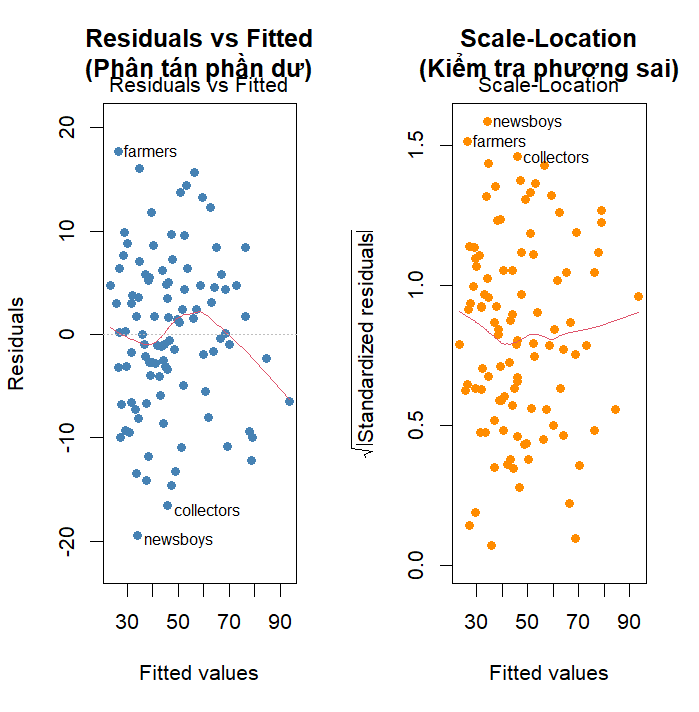
\includegraphics[width=0.82\textwidth]{./media/homoscedasticity_diagnostics.png}
  \caption{Chẩn đoán đồ thị cho mô hình \texttt{Prestige}. Residuals vs Fitted giúp kiểm tra mẫu hình phần dư; Scale-Location trực tiếp gợi ý độ phân tán phần dư có thay đổi theo giá trị khớp hay không.}
  \label{fig:homoscedasticity_prestige_diagnostics}
\end{figure}

Hình~\ref{fig:homoscedasticity_prestige_diagnostics} bổ sung bằng chứng trực quan: đường làm mịn trong Scale-Location không nằm ngang hoàn toàn và độ phân tán thay đổi theo vùng giá trị khớp. Điều này phù hợp với kết quả White test và biện minh cho bước kiểm tra suy diễn bằng sai số chuẩn vững.

\subsubsection{Hiệu Chỉnh Bằng HC3}

\begin{lstlisting}[style=Rstyle]
robust_model <- coeftest(model, vcov = vcovHC(model, type = "HC3"))
robust_model
\end{lstlisting}

\begin{lstlisting}[style=output]
               Estimate  Std. Error t value  Pr(>|t|)    
(Intercept) -6.84777872  3.25355462 -2.1047   0.03785 *  
income       0.00136117  0.00029942  4.5460 1.549e-05 ***
education    4.13744438  0.39588932 10.4510 < 2.2e-16 ***
\end{lstlisting}

\begin{center}
\small
\begin{tabular}{@{}lrrrr@{}}
\toprule
\textbf{Biến} & \textbf{Estimate} & \textbf{OLS SE} & \textbf{HC3 SE} & \textbf{HC3 p-value} \\
\midrule
Intercept & $-6.84778$ & $3.21898$ & $3.25355$ & $0.03785$ \\
\texttt{income} & $0.00136$ & $0.00022$ & $0.00030$ & $1.549\times 10^{-5}$ \\
\texttt{education} & $4.13744$ & $0.34891$ & $0.39589$ & $<2.2\times 10^{-16}$ \\
\bottomrule
\end{tabular}
\end{center}

Sau khi dùng HC3, sai số chuẩn của \texttt{income} và \texttt{education} đều tăng. Đây là dấu hiệu thường gặp khi SE cổ điển quá lạc quan dưới phương sai thay đổi. Tuy vậy, dấu hệ số và kết luận định tính không đổi: thu nhập và học vấn vẫn có quan hệ dương với điểm uy tín nghề nghiệp.

\begin{figure}[H]
  \centering
  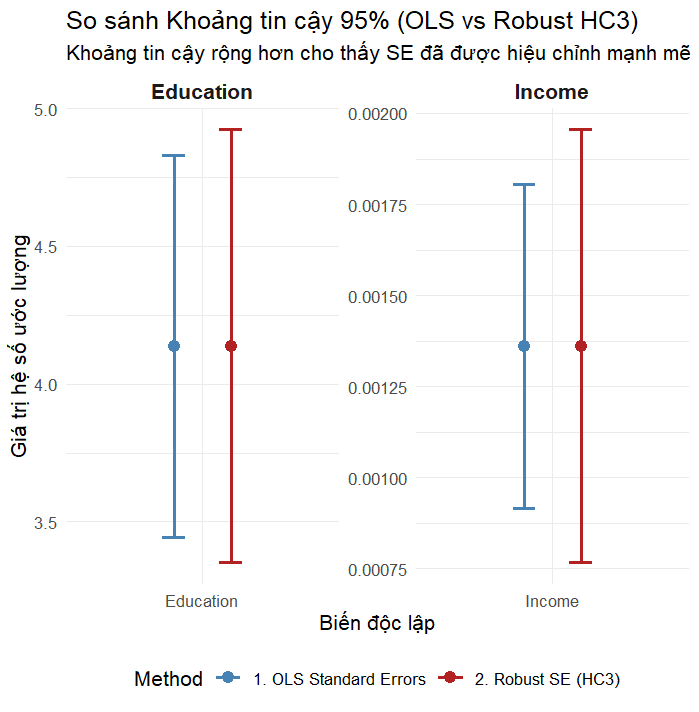
\includegraphics[width=0.82\textwidth]{./media/homoscedasticity_hc3_ci.png}
  \caption{So sánh khoảng tin cậy 95\% giữa OLS SE và HC3 robust SE. Điểm ước lượng giữ nguyên, nhưng khoảng tin cậy HC3 rộng hơn do độ bất định được hiệu chỉnh.}
  \label{fig:homoscedasticity_prestige_hc3_ci}
\end{figure}

Hình~\ref{fig:homoscedasticity_prestige_hc3_ci} nhấn mạnh điểm thực hành quan trọng: robust SE không thay đổi hệ số OLS, mà thay đổi cách đo độ bất định của hệ số. Vì các khoảng tin cậy HC3 vẫn nằm cùng phía so với $0$, kết luận về tác động dương của \texttt{income} và \texttt{education} vẫn ổn định.

\begin{notebox}
\textbf{Bài học từ Prestige.} Breusch--Pagan có thể không phát hiện phương sai thay đổi tuyến tính, trong khi White test và Scale-Location plot gợi ý cấu trúc phức tạp hơn. Khi nghi ngờ SE cổ điển, báo cáo HC3 giúp suy diễn thận trọng hơn mà vẫn giữ nguyên hệ số OLS.
\end{notebox}

% -----------------------------------------------------------------------------
